% Options for packages loaded elsewhere
\PassOptionsToPackage{unicode}{hyperref}
\PassOptionsToPackage{hyphens}{url}
%
\documentclass[
]{article}
\usepackage{amsmath,amssymb}
\usepackage{iftex}
\ifPDFTeX
  \usepackage[T1]{fontenc}
  \usepackage[utf8]{inputenc}
  \usepackage{textcomp} % provide euro and other symbols
\else % if luatex or xetex
  \usepackage{unicode-math} % this also loads fontspec
  \defaultfontfeatures{Scale=MatchLowercase}
  \defaultfontfeatures[\rmfamily]{Ligatures=TeX,Scale=1}
\fi
\usepackage{lmodern}
\ifPDFTeX\else
  % xetex/luatex font selection
\fi
% Use upquote if available, for straight quotes in verbatim environments
\IfFileExists{upquote.sty}{\usepackage{upquote}}{}
\IfFileExists{microtype.sty}{% use microtype if available
  \usepackage[]{microtype}
  \UseMicrotypeSet[protrusion]{basicmath} % disable protrusion for tt fonts
}{}
\makeatletter
\@ifundefined{KOMAClassName}{% if non-KOMA class
  \IfFileExists{parskip.sty}{%
    \usepackage{parskip}
  }{% else
    \setlength{\parindent}{0pt}
    \setlength{\parskip}{6pt plus 2pt minus 1pt}}
}{% if KOMA class
  \KOMAoptions{parskip=half}}
\makeatother
\usepackage{xcolor}
\usepackage[left = 2.5cm, right = 2.5cm, top = 2.5cm, bottom =
2cm]{geometry}
\usepackage{longtable,booktabs,array}
\usepackage{calc} % for calculating minipage widths
% Correct order of tables after \paragraph or \subparagraph
\usepackage{etoolbox}
\makeatletter
\patchcmd\longtable{\par}{\if@noskipsec\mbox{}\fi\par}{}{}
\makeatother
% Allow footnotes in longtable head/foot
\IfFileExists{footnotehyper.sty}{\usepackage{footnotehyper}}{\usepackage{footnote}}
\makesavenoteenv{longtable}
\usepackage{graphicx}
\makeatletter
\def\maxwidth{\ifdim\Gin@nat@width>\linewidth\linewidth\else\Gin@nat@width\fi}
\def\maxheight{\ifdim\Gin@nat@height>\textheight\textheight\else\Gin@nat@height\fi}
\makeatother
% Scale images if necessary, so that they will not overflow the page
% margins by default, and it is still possible to overwrite the defaults
% using explicit options in \includegraphics[width, height, ...]{}
\setkeys{Gin}{width=\maxwidth,height=\maxheight,keepaspectratio}
% Set default figure placement to htbp
\makeatletter
\def\fps@figure{htbp}
\makeatother
\setlength{\emergencystretch}{3em} % prevent overfull lines
\providecommand{\tightlist}{%
  \setlength{\itemsep}{0pt}\setlength{\parskip}{0pt}}
\setcounter{secnumdepth}{5}
\usepackage{float}
\usepackage{sectsty}
\usepackage{paralist}
\usepackage{setspace}\spacing{1.5}
\usepackage{fancyhdr}
\usepackage{lastpage}
\usepackage{dcolumn}
\usepackage{natbib}\bibliographystyle{agsm}
\usepackage[nottoc, numbib]{tocbibind}
\ifLuaTeX
  \usepackage{selnolig}  % disable illegal ligatures
\fi
\IfFileExists{bookmark.sty}{\usepackage{bookmark}}{\usepackage{hyperref}}
\IfFileExists{xurl.sty}{\usepackage{xurl}}{} % add URL line breaks if available
\urlstyle{same}
\hypersetup{
  hidelinks,
  pdfcreator={LaTeX via pandoc}}

\author{}
\date{\vspace{-2.5em}}

\begin{document}

\allsectionsfont{\raggedright}
\subsectionfont{\raggedright}
\subsubsectionfont{\raggedright}

\vspace{0cm}

\pagenumbering{gobble}

\begin{centering}

\Large

\doublespacing

\bf Thesis Report

\bf on

\bf FACTORS DETERMINING DIAMETER GROWTH OF SHOREA ROBUSTA (SAL)



\begin{center}\includegraphics[width=0.5\linewidth]{AFU_logo} \end{center}


\normalsize

\Large

\bf Agriculture and Forestry University


\bf Forestry Campus, Hetauda

\vspace{1cm}

\normalsize

\singlespacing

By

\vspace{0.5 cm}

\Large

\bf Binita Ghimire

\Large

\bf B.Sc. Forestry

\bf Fourth Year (Second Semester)

\vspace{1cm}

\normalsize

2023-08-17

\end{centering}

\newpage

\pagenumbering{roman}
\newpage
\fontsize{12}{18}
\tableofcontents

\newpage

\listoftables
\listoffigures

\newpage

\clearpage
\pagenumbering{arabic}
\fontsize{12}{18}

\hypertarget{methodology}{%
\section{Methodology}\label{methodology}}

\hypertarget{study-area}{%
\subsection{Study Area}\label{study-area}}

\hypertarget{source-of-data}{%
\subsection{Source of Data}\label{source-of-data}}

\hypertarget{data-analysis}{%
\subsection{Data analysis}\label{data-analysis}}

\hypertarget{results}{%
\section{Results}\label{results}}

Tree diameter growth from different permanent sample plots.

\hypertarget{correlation-for-feature-selection}{%
\subsection{Correlation for Feature
Selection}\label{correlation-for-feature-selection}}

Correlation method is simplest method, widely used for the variables
having linear relationship, feature selection for modelling.

\begin{longtable}[]{@{}lr@{}}
\caption{Correlation of different features to basal area
growth}\tabularnewline
\toprule\noalign{}
Features & correlation coefficient \\
\midrule\noalign{}
\endfirsthead
\toprule\noalign{}
Features & correlation coefficient \\
\midrule\noalign{}
\endhead
\bottomrule\noalign{}
\endlastfoot
tree\_density & 0.50 \\
min\_temperature & -0.17 \\
max\_temperature & -0.16 \\
crown\_cover & 0.16 \\
elevation\_nepal & 0.15 \\
aspect & 0.15 \\
ba\_ha\_old & 0.14 \\
lat & 0.13 \\
organic\_layer\_thickness & 0.12 \\
precipitation\_accumulation & 0.12 \\
lon & -0.10 \\
slope.map\_nepal & 0.09 \\
climate\_water\_deficit & -0.08 \\
wind\_speed\_at\_10m & -0.07 \\
palmer\_drought\_sensitive\_index & 0.06 \\
organic\_layer\_type & 0.04 \\
soil\_moisture & 0.03 \\
soil\_depth & -0.01 \\
penetration\_depth & 0.00 \\
\end{longtable}

\hypertarget{stepwise-regression}{%
\subsection{Stepwise Regression}\label{stepwise-regression}}

This method involves fitting a regression model with all potential
predictor variables and then alliteratively adding or removing variables
based on their significance until an optimal subset is obtained.

\begin{figure}
\centering
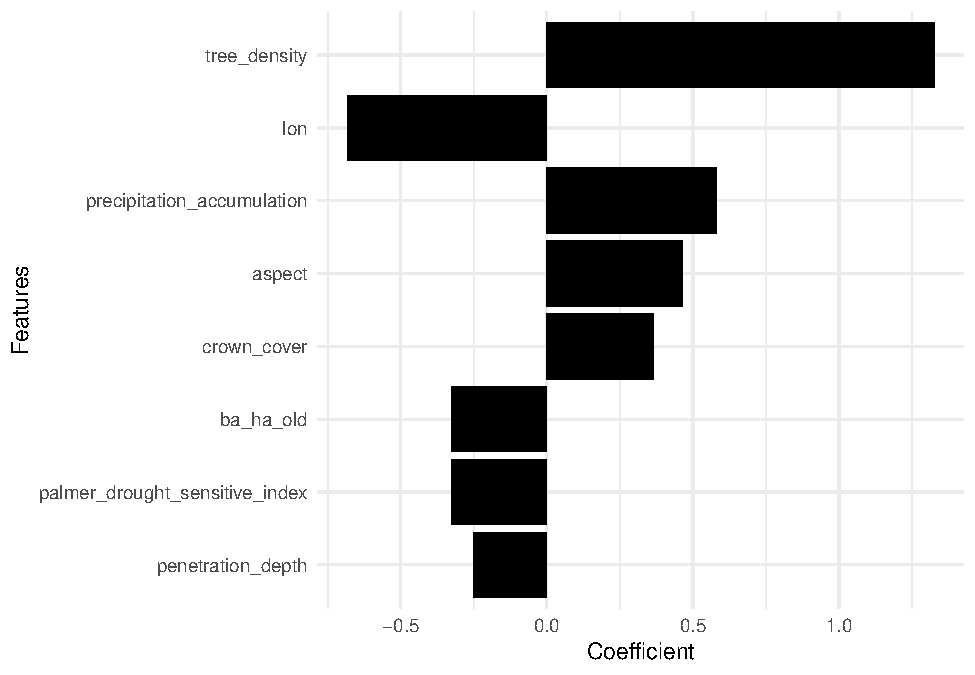
\includegraphics{feature_selection_report_files/figure-latex/unnamed-chunk-4-1.pdf}
\caption{Feature and thier coefficients(in modulus) in order}
\end{figure}

\hypertarget{low-variance-filtering}{%
\section{Low variance filtering}\label{low-variance-filtering}}

The feature selection method ``removing the factors having the lowest
variability,'' is commonly known as ``low variance filtering'' or
``constant feature removal.'' It is a straightforward technique used to
eliminate features with very little or no variability in their values.
In the context of feature selection, features with low variance do not
contribute much information to the model because their values remain
almost constant across all observations or samples. Such features are
less likely to provide meaningful insights and might even add noise to
the model, potentially leading to over fitting.

\begin{longtable}[]{@{}lr@{}}
\caption{Results from low variance filtering}\tabularnewline
\toprule\noalign{}
Variables & Coefficient of variables \\
\midrule\noalign{}
\endfirsthead
\toprule\noalign{}
Variables & Coefficient of variables \\
\midrule\noalign{}
\endhead
\bottomrule\noalign{}
\endlastfoot
organic\_layer\_type & 150.94 \\
organic\_layer\_thickness & 111.44 \\
slope.map\_nepal & 97.81 \\
tree\_density & 89.33 \\
aspect & 81.68 \\
elevation\_nepal & 62.67 \\
palmer\_drought\_sensitive\_index & 62.53 \\
penetration\_depth & 46.44 \\
ba\_ha\_old & 39.48 \\
soil\_moisture & 39.07 \\
precipitation\_accumulation & 26.83 \\
crown\_cover & 26.42 \\
soil\_depth & 21.57 \\
climate\_water\_deficit & 21.28 \\
min\_temperature & 9.51 \\
max\_temperature & 6.66 \\
wind\_speed\_at\_10m & 4.07 \\
lon & 2.54 \\
lat & 2.42 \\
\end{longtable}

\hypertarget{multicollinearity-test}{%
\subsection{Multicollinearity Test}\label{multicollinearity-test}}

\begin{longtable}[]{@{}lr@{}}
\caption{Selected variables with thier VIF values}\tabularnewline
\toprule\noalign{}
variable & VIF values \\
\midrule\noalign{}
\endfirsthead
\toprule\noalign{}
variable & VIF values \\
\midrule\noalign{}
\endhead
\bottomrule\noalign{}
\endlastfoot
aspect & 1.32 \\
tree\_density & 1.43 \\
organic\_layer\_type & 1.54 \\
organic\_layer\_thickness & 1.66 \\
crown\_cover & 1.70 \\
wind\_speed\_at\_10m & 1.70 \\
ba\_ha\_old & 1.74 \\
penetration\_depth & 1.79 \\
\end{longtable}

\hypertarget{randomforest-regressor}{%
\subsection{RandomForest Regressor}\label{randomforest-regressor}}

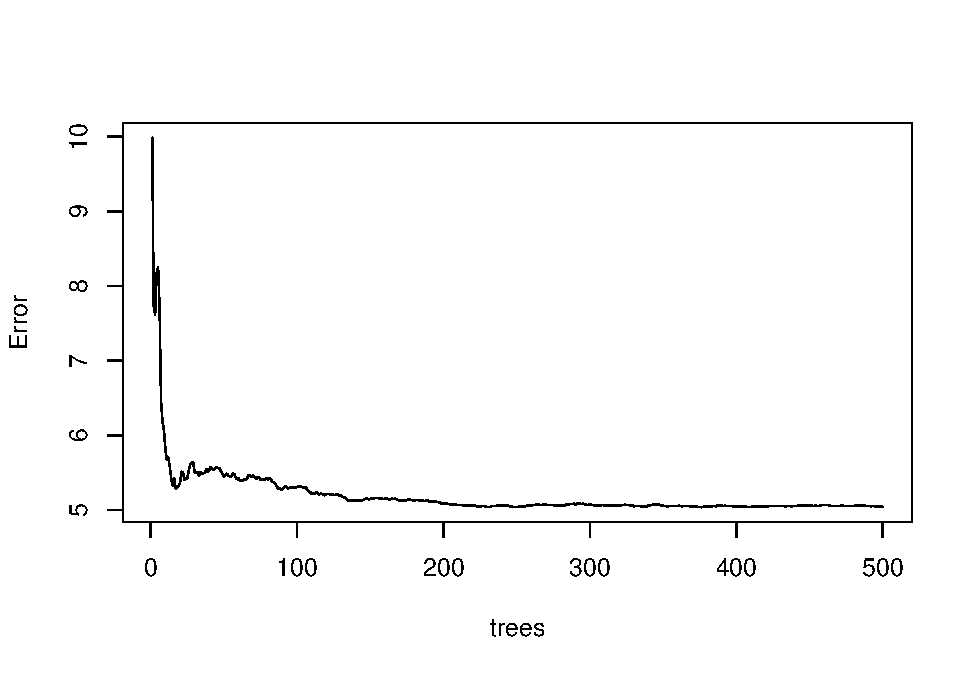
\includegraphics{feature_selection_report_files/figure-latex/unnamed-chunk-9-1.pdf}

\begin{longtable}[]{@{}lr@{}}
\caption{Importance of feature in the model}\tabularnewline
\toprule\noalign{}
Features & IncNode Purity Value \\
\midrule\noalign{}
\endfirsthead
\toprule\noalign{}
Features & IncNode Purity Value \\
\midrule\noalign{}
\endhead
\bottomrule\noalign{}
\endlastfoot
tree\_density & 264.713795 \\
ba\_ha\_old & 89.201379 \\
penetration\_depth & 71.913346 \\
lat & 71.604930 \\
min\_temperature & 57.178158 \\
lon & 55.333382 \\
wind\_speed\_at\_10m & 53.999507 \\
soil\_moisture & 53.205255 \\
crown\_cover & 52.048419 \\
max\_temperature & 51.911490 \\
elevation\_nepal & 50.208452 \\
palmer\_drought\_sensitive\_index & 46.548952 \\
slope.map\_nepal & 44.020634 \\
climate\_water\_deficit & 43.623167 \\
precipitation\_accumulation & 42.737837 \\
organic\_layer\_thickness & 11.401235 \\
soil\_depth & 10.999894 \\
aspect & 9.834277 \\
organic\_layer\_type & 9.390413 \\
\end{longtable}

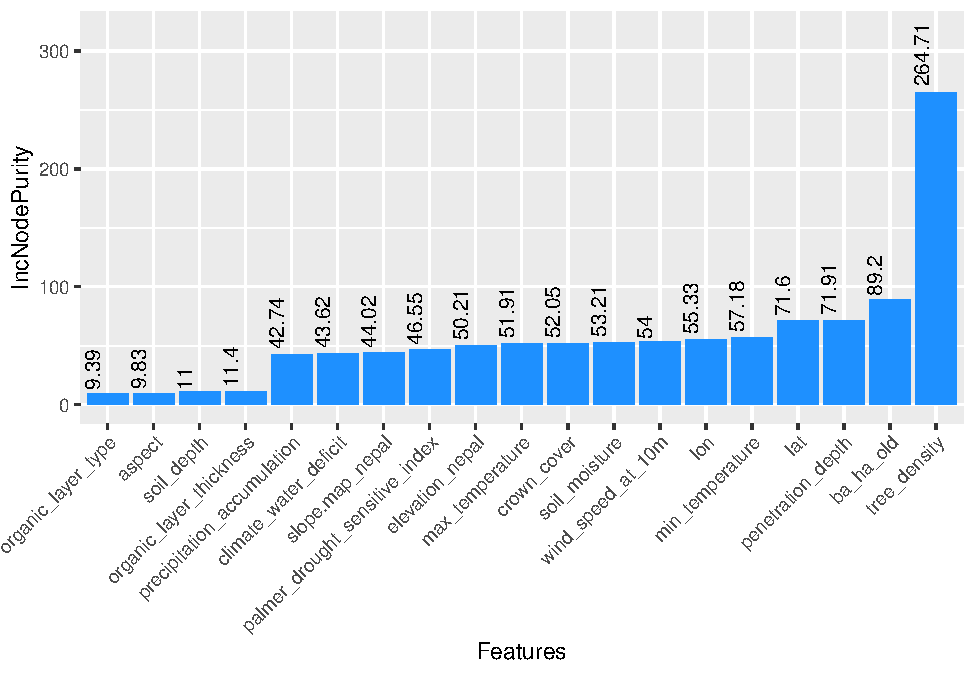
\includegraphics{feature_selection_report_files/figure-latex/unnamed-chunk-11-1.pdf}

\end{document}
